\section{Puesta en marcha del sistema}

En esta sección se describirán las acciones necesarias para poner en marcha el sistema en un entorno Windows, haciendo uso del subsistema Windows para ejecutar un agente Microros conectado al dispositivo por medio de una conexión USB-Serial.


\subsection{Actuaciones en Powershell de Windows}

Para poner en marcha el proyecto primero hay que montar el setup de ROS2 en Powershell de la siguiente forma:

\begin{verbatim}
C:\dev\ros2\_humble\local\_setup.ps1
\end{verbatim}

Y abrir el proyecto de Unity en la misma Powershell

\begin{verbatim}
unity.exe -projectPath "D:\Unity\Unity Projects\Thesis-Unity-Pan-Tilt\"
\end{verbatim}

Luego usar el programa usbipd para atar los puertos correspondientes a WSL2 (véase sección \ref{WLS-considerations})
En este paso hay que asegurarse de que ya estamos conectados al WiFi del ESP32 (véase la figura \ref{figure:usbipd-in-the-lan})

\begin{figure}[!htb]
   \centering
    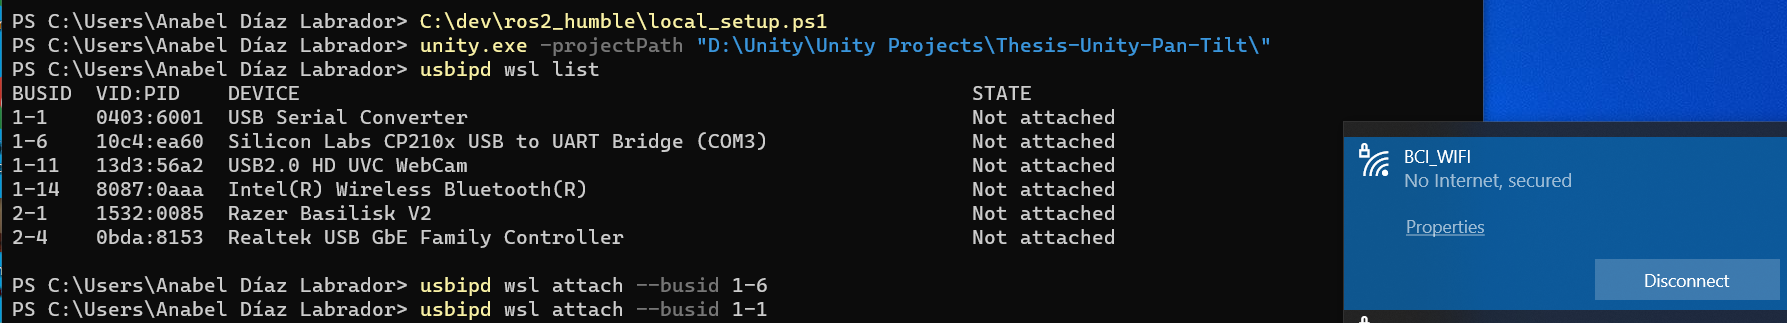
\includegraphics[width=0.8\linewidth]{figures/usbipd-in-the-lan.png}
   \caption{Preparación del proyecto en Windows}
   \label{figure:usbipd-in-the-lan}
\end{figure}

El comando para atar el puerto a WSL2 con usbipd es:

\begin{verbatim}
usbipd wsl attach --busid BUSID
\end{verbatim}

Donde BUSID es el busid correspondiente.

\subsection{Actuaciones en Ubuntu sobre WSL2}

\subsubsection{Agente de micro-ROS}

En una terminal de WSL2 hay que dar permisos a los puertos, por ejemplo si hemos atado el microcontrolador y la cámara (esta \'ultima solo en caso de que sea necesario su monitorizaci\'on) sería así:

\begin{verbatim}
sudo chmod 777 /dev/ttyUSB0
sudo chmod 777 /dev/ttyUSB1
\end{verbatim}

Se realiza ahora un source install/setup.bash del repositorio del agente de microros (véase el apéndice \ref{section:microrosagent}), para hacer que esta aplicaci\'on est\'e disponible para ROS2.

Finalmente, ejecutamos el agente de micro-ROS poniendo el puerto correspondiente:

\begin{verbatim}
ros2 run micro_ros_agent micro_ros_agent serial --dev /dev/ttyUSB0
\end{verbatim}


\subsubsection{Monitorizaci\'on de la cámara}

En otra terminal de WSL2 se necesita establecer como entorno de desarrollo ``esp-idf v4'' haciendo un source al script de exportaci\'on de esta versi\'onde la toolchain (v\'ease  \ref{section:cameraenvironmentinstallation}) 

\begin{verbatim}
get_idf4
\end{verbatim}

Primer es necesario compilar el firmware e introducirlo en el microcontrolador

\begin{verbatim}
idf.py build
idf.py -p /dev/ttyUSB1 flash
\end{verbatim}

Luego se puede monitorear de la siguiente manera:

\begin{verbatim}
idf.py -p /dev/ttyUSB1 monitor
\end{verbatim}


\section{Funcionamiento del prototipo}
\label{section:prototype-working}
El sistema presenta una interfaz intuitiva y directa. Su funcionamiento sigue un esquema de ``apunta y dispara'', donde el usuario debe centrar el código QR en un cuadrado designado como punto de mira en la interfaz de la cámara. Seis rectángulos ubicados en la parte inferior del HUD de la cámara se iluminan en verde al detectar códigos QR.



Incorpora cuatro NeuroButtons (véase sección \ref{subsubsection:add-neurotag}) que controlan el movimiento del sistema Pan-Tilt en cuatro direcciones: arriba, abajo, izquierda y derecha. El HUD de la cámara, ubicado centralmente, alberga un cuadrado que permanece constantemente en rojo, cambiando a verde cuando se detecta exitosamente un código QR. Se puede ver prototipo entero conectado y montado en la figura \ref{figure:prototipo-working}.

\begin{figure}[!htb]
   \centering
    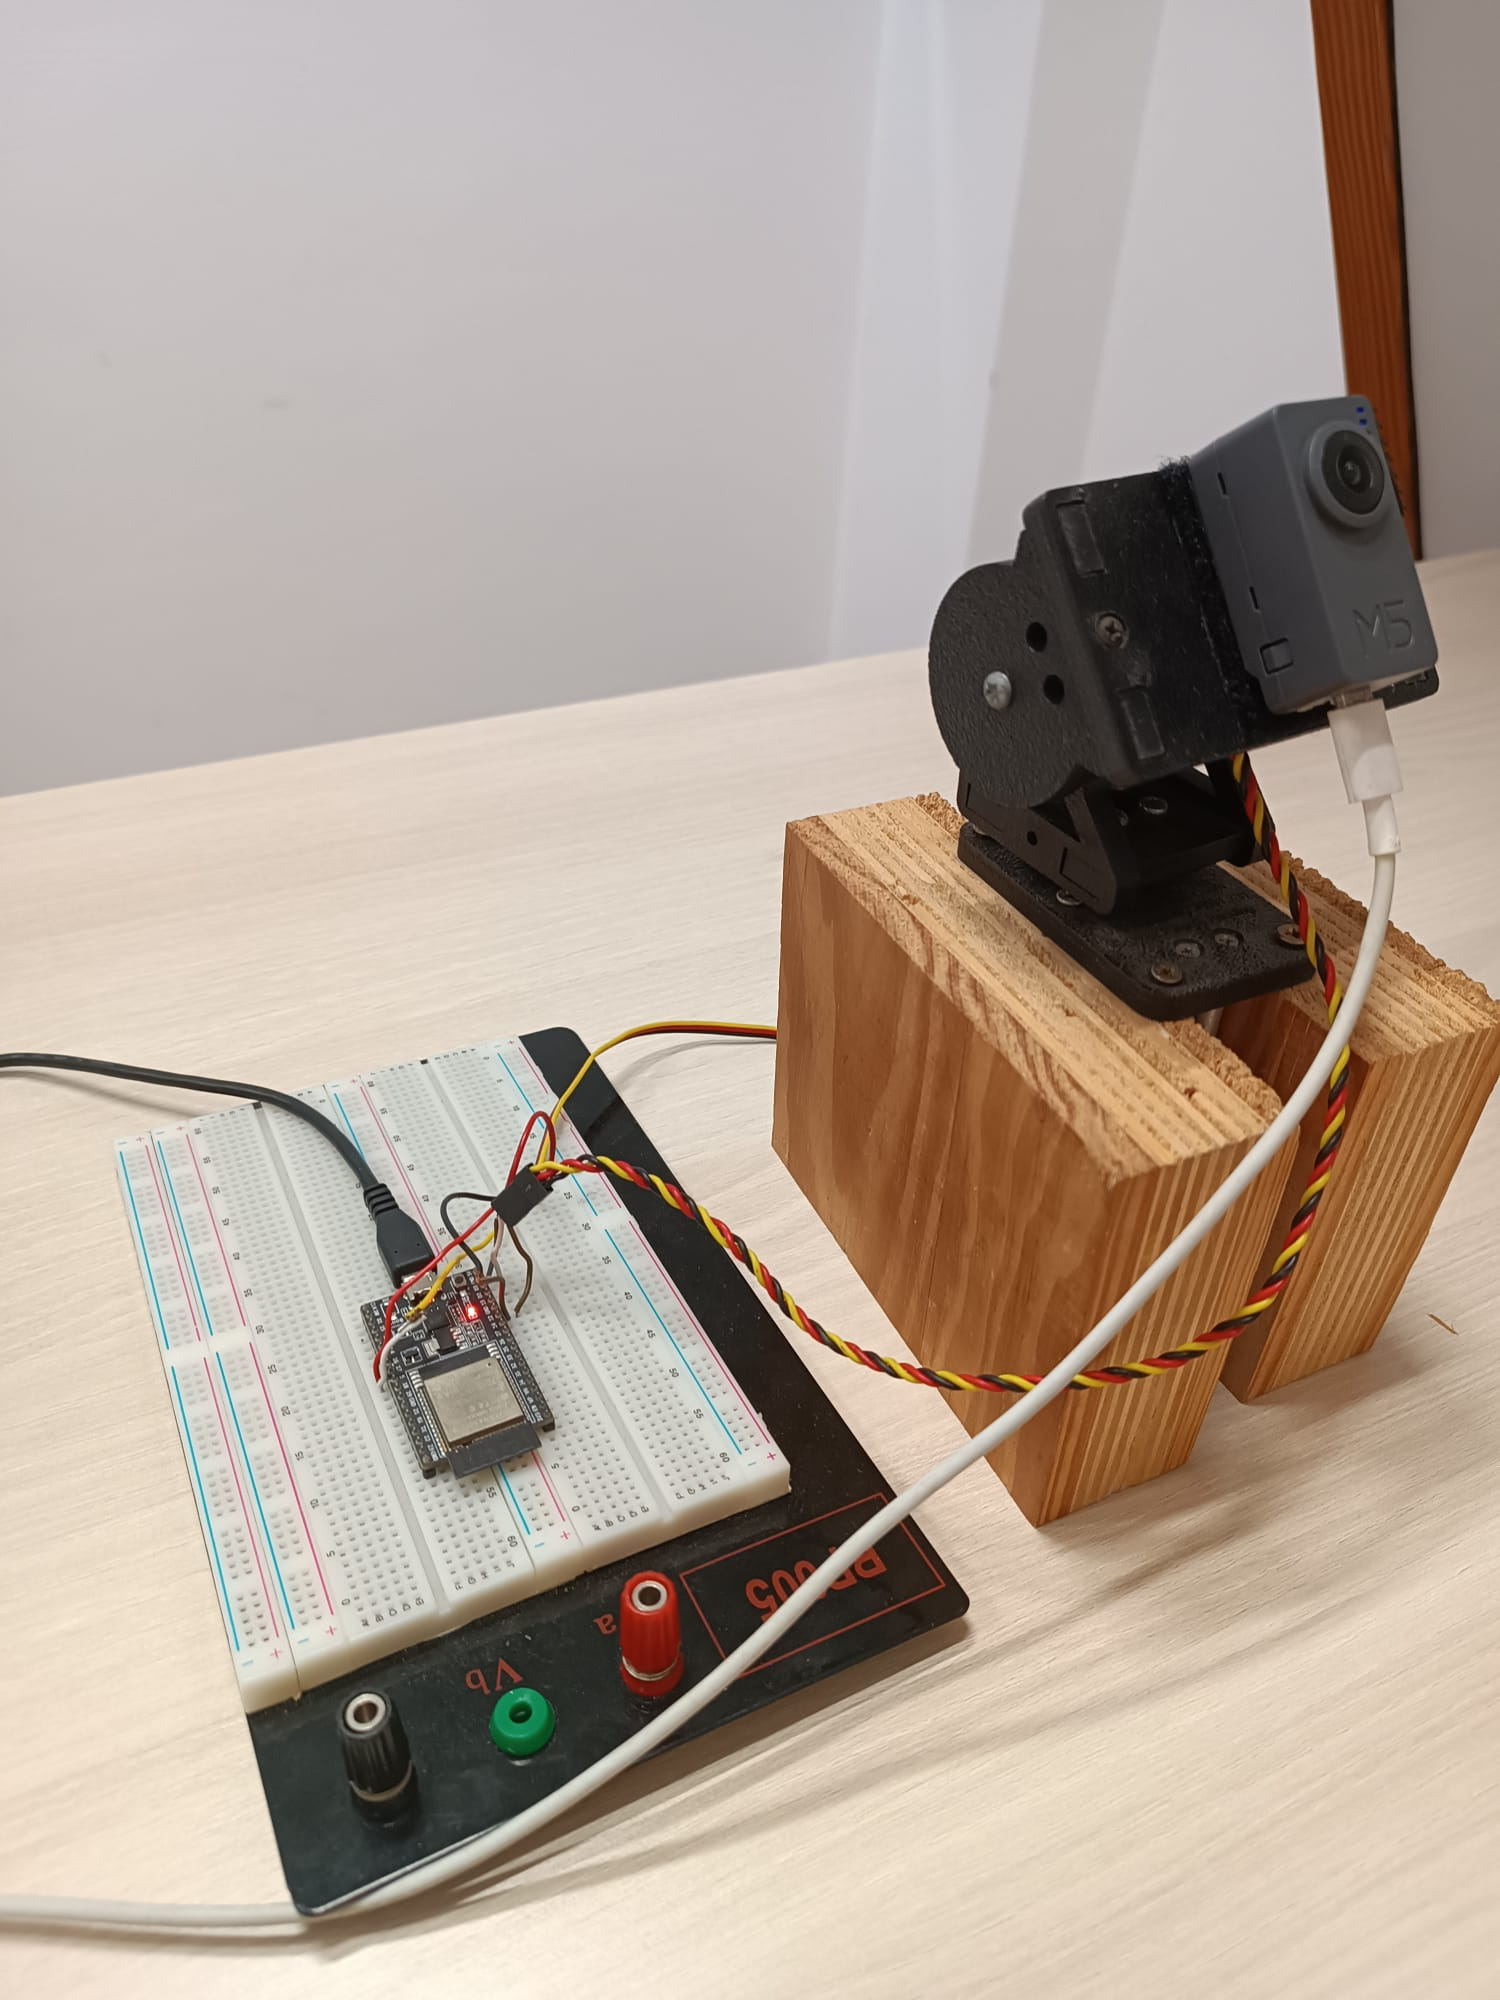
\includegraphics[width=0.35\linewidth]{figures/prototipo.jpg}
   \caption{Prototipo montado y conectado}
   \label{figure:prototipo-working}
\end{figure}